\documentclass{article}
\usepackage[utf8]{inputenc}
\usepackage{amsthm}
\usepackage{amsmath}
\newtheoremstyle{mystyle}% name
  {\topsep}% Space above
  {\topsep}% Space below
  {\normalfont}% Body font
  {}% Indent amount
  {\bfseries}% Theorem head font
  {}%Punctuation after theorem head
  {.5em}%Space after theorem head
  {}% theorem head spec
\theoremstyle{mystyle}
\newtheorem{prob}{Problem}
\usepackage{graphicx}
\usepackage{wrapfig}
 %preamble
\title{EN.520.214 Project 1}
\author{LJ Gonzales}
\date{March 2023}

\begin{document}
\maketitle
\section{Part 0: Code hyperparameters}
	To verify the result of each part, the user need only change a few hyperparameters at the beginning of the code.
	\begin{enumerate}
		\item The \emph{use\_fake\_message} boolean tells the program whether to run the following steps with the loaded message or a fabricated letter string/bit string. Set to false for part I and II, true for part III.
		\item The \emph{real\_message} string, if \emph{use\_fake\_message} is set to true, corresponds to the name of the real signal to analyze. Set to "SonarEcho" for part I, "ReceivedSignal" for part II, either one for part III. Make sure to have used \emph{load ReceivedSignalX} for the signal number to be analyzed.
		\item The \emph{echo} bool decides whether the output is the distance to the located object, or the program's best try at a translate message. Set to true for part I, false for part II and III.
		\item The \emph{tolerance} value is a parameter used in getting the distance traveled by the echo. Set to 1 to make sure that only the highest amplitude of the received signal is considered in the echo, but \emph{make sure to set to 0 for parts II and III}
		\item \emph{string\_to\_check} is the control string for which to evaluate the robustness of the signals.
		\item \emph{fake\_message} is used for \emph{use\_fake\_message} set to true in parts III, and as a ground truth for testing parts I and II. When checking robustness, acts as a superparameter to translate the letter string to a bitstring and should not be changed, but can be changed to a non-ASCII bitstring in the form [1 0 0 1...] etc.
		\item \emph{code\_type} is, as the name implies, the type of code to create the amplitude-time signal from the \emph{fake\_message} bitstring. Set to 't' for part II, leave alone otherwise (the robustness evaluator iterates through all ping types anyway).
		\item Finally the \emph{run\_signal\_comparison} boolean outputs the results of part III signal comparison code. While running, the function clutters the screen so it is recommended to do this in the last step.
	\end{enumerate}
\section{Part 1}
	Note that after having decoded the message, finding the distance between the ship and the located object becomes a trivial task: we can just find the time upon which the echo is heard (number of samples multiplied by $\frac{1}{\text{samples per second}}$) and multiply that by the speed of propagation inside the medium, given at $5000$ feet per second. \\
	We visualize what is in the code in a 3 step process (Figure \ref{3stepfakecode} shows an example with a message fabricated with the \emph{makemessage()} function, which takes in a bitstring, a ping, and a method of how to take its complement ('f' for flip or 'i' for invert), and outputs the corresponding amplitude-time signal. Figure \ref{3steprealcode} shows a similar procedure, instead using the actual echo to be heard).
	We 1) plot the message to be decoded, 2) it being convolved with the original ping signal, and 3) our best attempt at a reconstructed message, given the output of the matched filter.
\begin{figure}[h]
	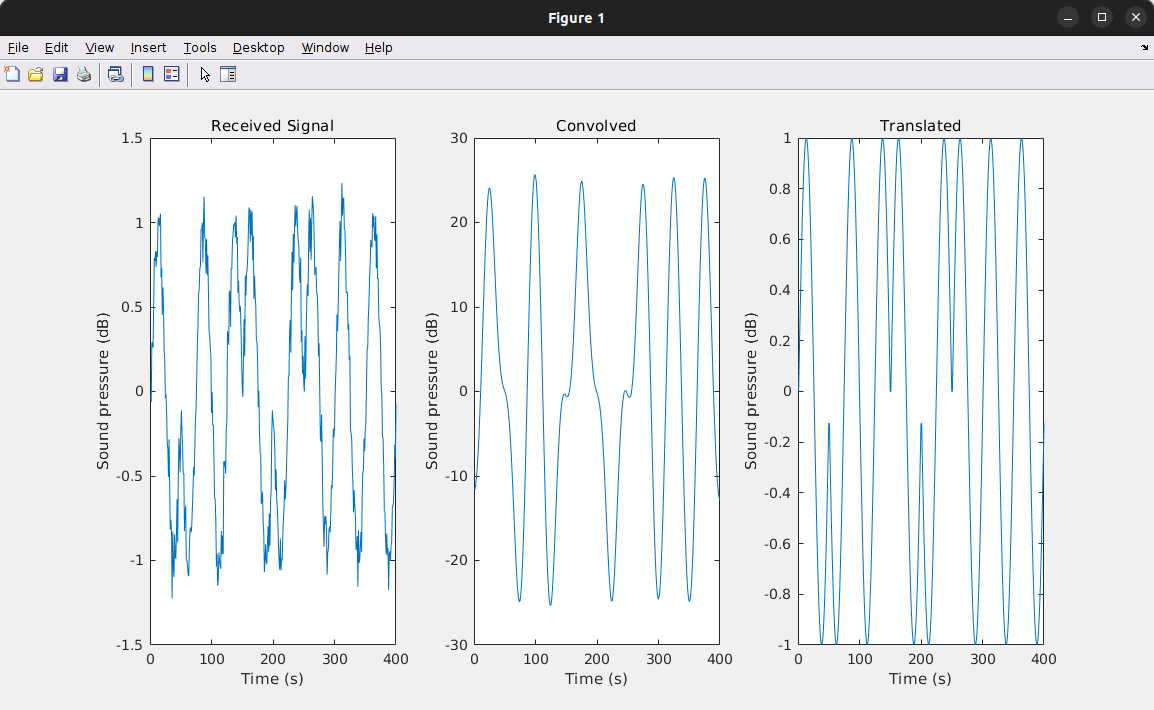
\includegraphics[width =\textwidth]{3stepfakecode.png}
	\label{3stepfakecode}
	\caption{a) Received, b) Convolved, and c) Interpreted from convolved with dummy message}
\end{figure}
\begin{figure}[h]
	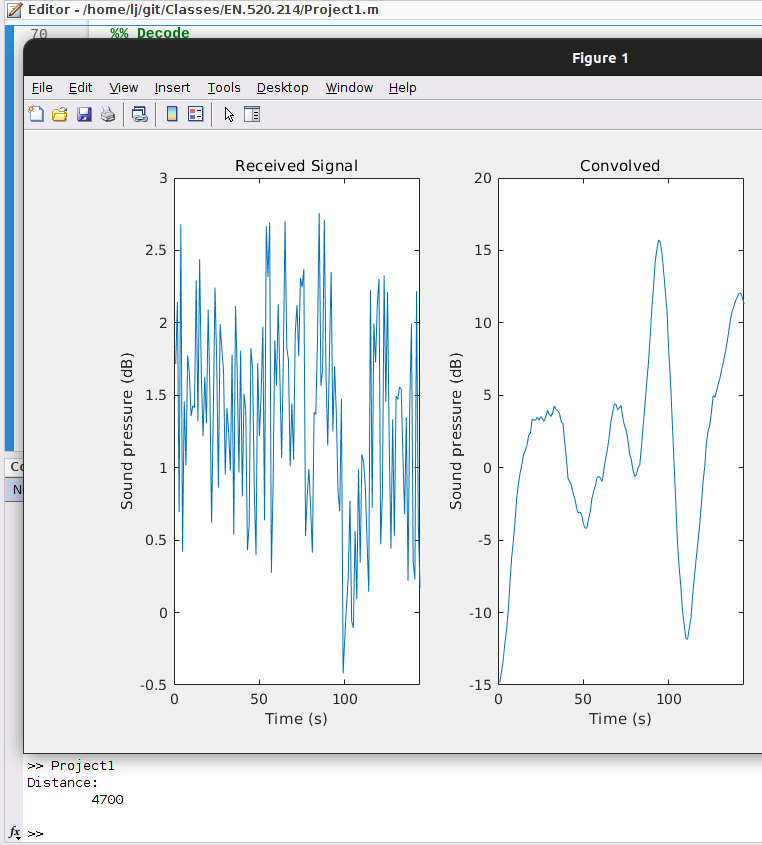
\includegraphics[width =0.5\textwidth]{3steprealcode.png}
	\label{3steprealcode}
	\caption{Same as previous, with SonarEcho. Distance is output to the terminal} 
\end{figure}

	Our test with the fake, non-noisy code best illustrates that when the bipolar signal is in its low state, the convolution reaches a peak low, and a peak high in its high state. This is consistent with our understanding of what the convolution operation does in terms of overlapping sums.
	Note that in order to convolve the message with Matlab's \emph{convolve}, we needed to provide the ping flipped over the time axis and shifted by one period. However, because the ping begins at 0 in the provided file, the \emph{fliplr} function does both of these simultaneously.
	To evaluate the contents of the message, we need to divide it in equal intervals of length $\text{length(SonarPing)}$.
	The problem is that we do not know \emph{a priori} how to do this, because the time between sending and receiving is not necessarily an integer multiple of the length of the code, depending on how far the object is that reflected it.
	We know, however, that the recording \emph{does} contain the reflected signal (a positive 1) at least once inside it, and that any further communications (if any) are sent without any delay from the first. We can then find the global maximum of the convolved graph and center it accordingly.
	Note that here we are making a non-evident assumption about noise contamination in the signal: We need
	\[
	\int_{t}^{t+T}(p(t))^2dt \geq \int_{t}^{t+T}p(t)n(t)dt \text{  } \forall \text{  } t
	.\] 
That is, the overlap of the ping should not be less than the overlap of the noise and ping at any given time.
This is not straightforward to prove without knowing both the amplitude and frequency of the noise contamination, so we can get around proving this requirement by making the further assumption that the noise frequency is much higher than the ping frequency:
we can then use the fact that this particular signal is symmetric around 0 in amplitude, making the right hand side of the above equation approximately 0 for any choice of t 
(the overlap on the positive half of the ping averages out to be equal and opposite to the overlap on the negative side).
In practice, if we don't have a positive-negative symmetric signal, as in the following parts, we can also ignore this requirement by making the ping amplitude much larger than the worst-case noise amplitude, and we will see that ping types that are not symmetric around 0, tend to perform a bit worse, at least with this additive noise.

All in all, we find the reflected signal to be 4700 feet away from the source. Note that in the reconstructed message (rightmost subplot in figure \ref{3steprealcode}), we observe what looks like a 0 bit in the very first position. This might be the recording apparatus sensing the transmitted signal as it is being produced. Our distance calculator gets around this by knowing that this 0 will be reflected (if it comes back), hence it knows to wait only for a 1 bit (global max) in the convolved.
\section{Part II}
We have in the code divided the task of decoding the signal into multiple helper function, centered around the \emph{evaluate} function which takes in a convolved recording and iterates through batches of length corresponding to the ping signal known prior.

It then outputs a binary array, with one bit per processed batch, whose parity depends on whether the first point in the batch was greater than or lower than 0.
While trying to strengthen the robustness of the match filter to high-noise inputs, we decided to introduce a threshold parameter \emph{thresh}, defaulting at 0.3, which instead of taking the sign of the first or middle point in the data batch, makes the match filter consider only the first point with magnitude $\geq \text{thresh}\times A_{max}$, where $A_{max}$ is the global maximum of the absolute value of the signal. If no such point is found (which can occur in very high noise signals), the matched filter returns the mode of the sign of the batch (i.e if the signal is \emph{mostly} positive throughout the batch, a 1 is assumed, etc.) \\

Increasing the threshold constant makes the receiver less sensitive to noise, extending its maximum range, but may result in loss of information. This feature could be used to locate a faraway submarine first, before getting closer to it for more intricate communication.\\

We also note the use of the \emph{char} operator instead of the use of a lookup table to decode the message. Matlab, and indeed mostscripting languages, support the transformation of integers to ASCII using a local lookup table without the need for an extension. We still include the code for a manual lookup for completion, in case we wanted to use this script for non-ascii encodings, for security purposes.

The messages sent were \emph{SOS, Help!}, and \emph{Nevermind}.

\section{Part III}
Figure \ref{miccheck} shows the noisy, convolved, and translated interpretation (the original signal back) of the string 'mic check mic check'.
\begin{figure}[h]
	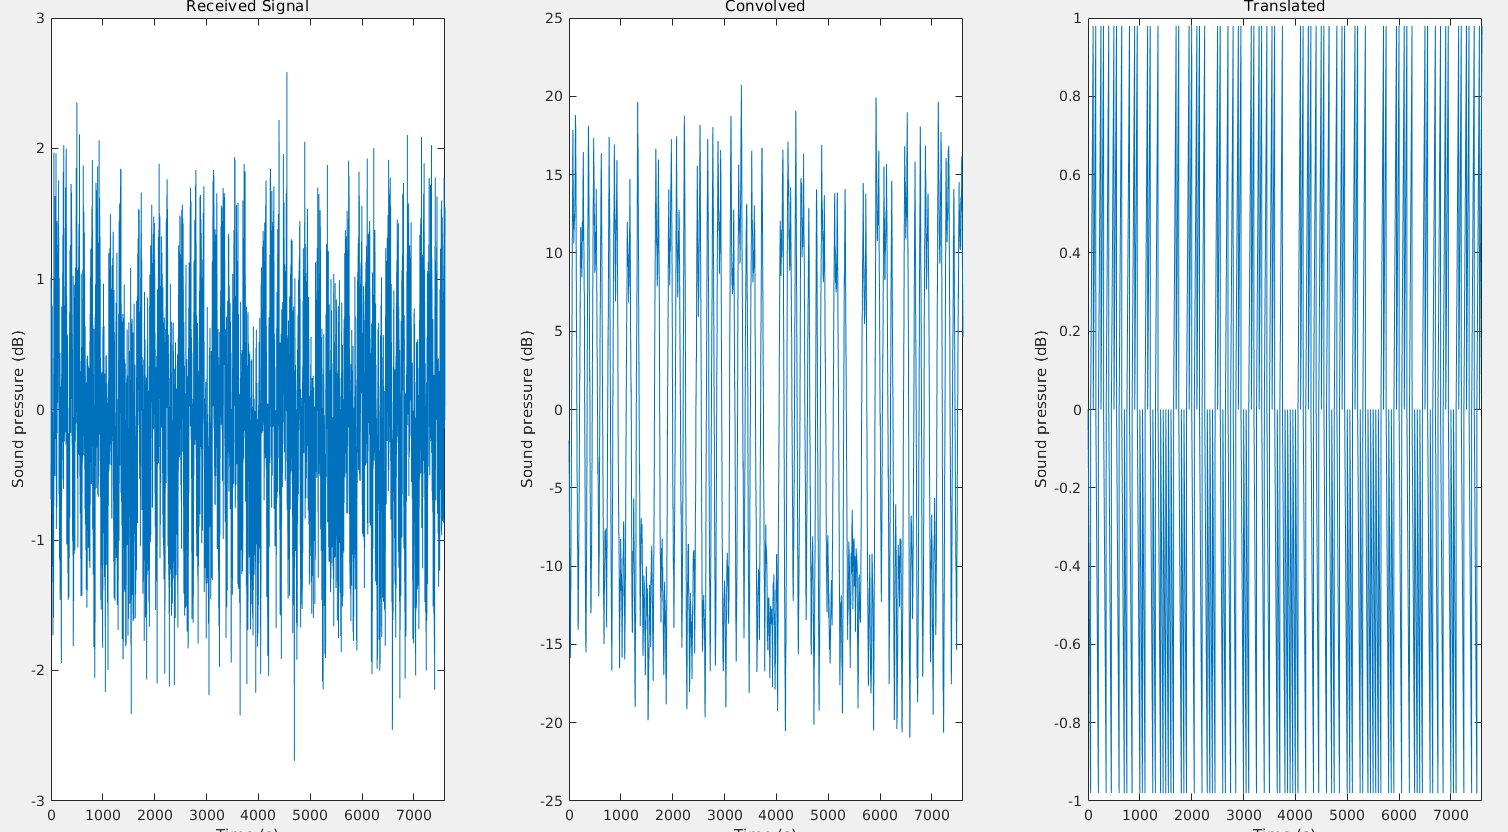
\includegraphics[width =\textwidth]{miccheck.png}
	\label{miccheck}
	\caption{3-step translation of 'mic check mic check'}
\end{figure}
\begin{figure}[h]
	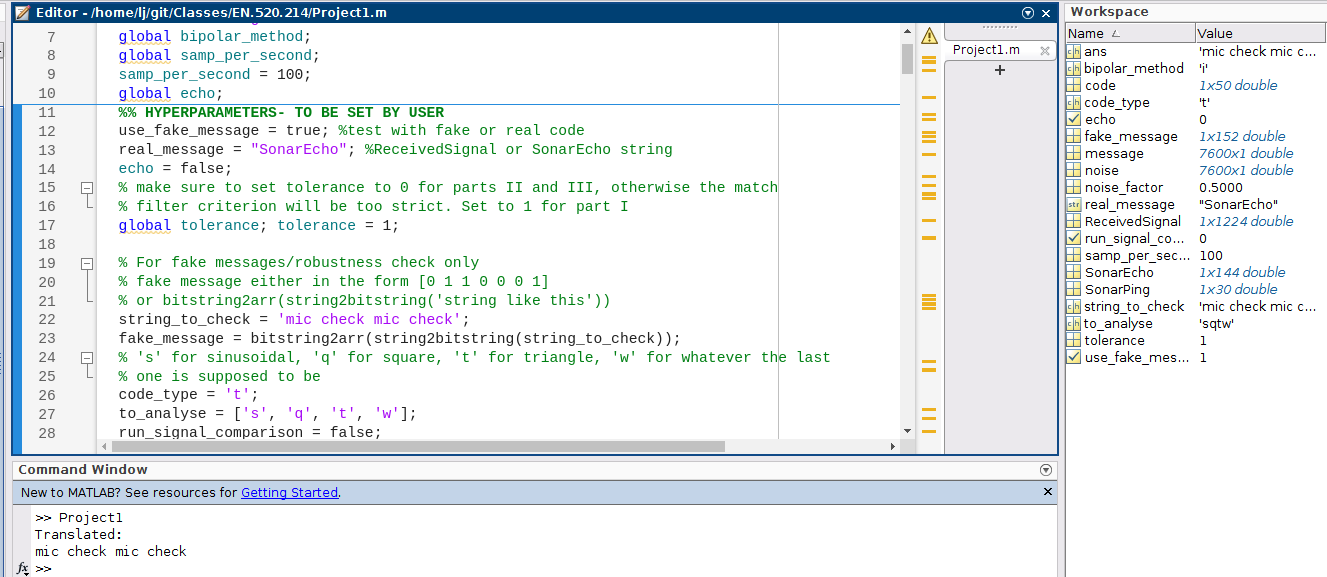
\includegraphics[width =\textwidth]{output.png}
	\label{output}
	\caption{String before noising and interpreted output. Additive noise with amplitude up to 110\% the original signal amplitude was possible with no distortion of this long string, showing the utility of match filters}
\end{figure}


We can combine all the functions used earlier to create a ping evaluator, also linked in the code.
It progressively increases the noise factor to the message \emph{"mic check mic check"}, translates it to a signal, and uses the above steps to decode it again. Once it gets at least one character -equivalently, a bit- wrong, it returns the boundary noise factor as the result of the evaluation.
Figure \ref{sensitivities} shows the output of this function when the noise factor was incremented by 0.01 per iteration. If more precision is necessary we can reduce this step factor.

Note that this is not necessarily an indicator of the maximum amount of noise that the signal can take: most signals had sucessful trials at noise levels up to 100\% of the original signal amplitude or more. They were just not able to do so reliably under the hundreds of passes of the evaluator.
To get a more holistic representation of reliability, the code could be changed to allow up to \emph{n} bit flips in a single pass, or give more than 1 try to get the signal right. This will depend on specific applications: here we assume one-shot communication.
Also note that the string used throughout testing was quite long: \emph{"mic check mic check"}, and a single error in any letter was considered a failure of the pass. In reality, a communication signal would include lots of redundancy and clever methods to make sure that just a single bit flip could still be translated clearly.

We will note that the signals which tended to perform better were the ones that maximized $\int_{T}p(t)p'(t)dt$, where $p(t)$ is the ping and $p'(t)$ its converse. just as we had predicted initially.
For example, the square signal has an area of 1, so its overlap with itself is 1, while the triangular signal has an area of $\frac{1}{2}$, such that its area is $\frac{1}{4}$, and their relative ordering on the score chart reflects this. We show in figure \ref{pings} the four signals to illustrate this.

\begin{figure}[h]
	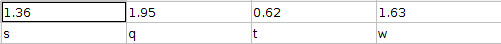
\includegraphics[width =\textwidth]{sensitivities.png}
	\label{sensitivities}
	\caption{Robustness score of each given signal. s for sinusoidal, q for square, t for triangle, and w for the last one}
\end{figure}
\begin{figure}[h]
	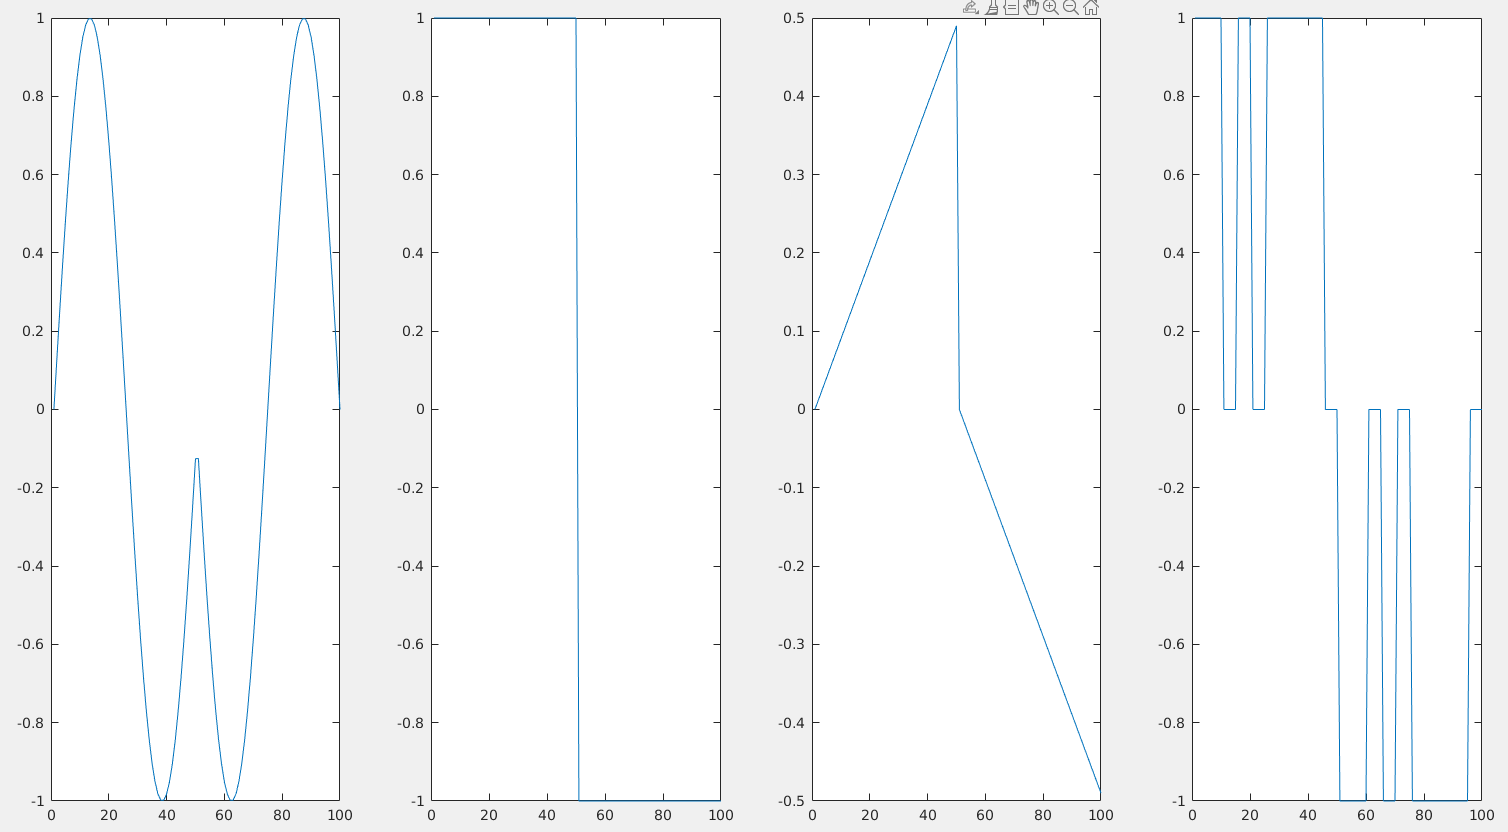
\includegraphics[width =\textwidth]{pings.png}
	\label{pings}
	\caption{Messages iterated over in robustness evaluator function}
\end{figure}

\end{document}
